\chapter{扩散}
    \section{扩散的微观机制}
        扩散的微观机制有四种,分别是\textbf{间隙扩散}\index{间隙扩散}、\textbf{环形扩散}\index{环形扩散}、\textbf{空位扩散}\index{空位扩散}、\textbf{挤列扩散}\index{挤列扩散}
        \subsection{间隙扩散}
            目前对于间隙扩散根据间隙原子尺寸分为两种情况考虑,可以有两种机制,分别是直接间隙机制和推填机制。

            对于尺寸较小的间隙原子,从一个间隙位置跳到相邻的空着的间隙位置,
            称为\textbf{直接间隙机制}\index{间隙扩散!直接间隙机制}。

            如果间隙原子尺寸较大,很难从一个间隙位置跳到另一个间隙位置,因为跳跃会造成很大的瞬时畸变能。
            因此提出另一种可能的扩散方式:位于间隙位置的原子把它位于最近邻的正常点阵
            位置的原子推入间隙位置,而自己占据该位置,这个机制称为\textbf{推填机制}\index{间隙扩散!推填机制},
            也称为\textbf{间接间隙机制}\index{间隙扩散!间接间隙机制}。
        \subsection{环行扩散}
            \textbf{环行扩散}\index{环行扩散}分为两种,分别是\textbf{直接交换}\index{环形扩散!直接交换}和\textbf{循环交换}\index{环形扩散!循环交换},
            具体过程如\autoref{环行扩散的两种机制}所示。
            \begin{figure}[ht]
                \centering
                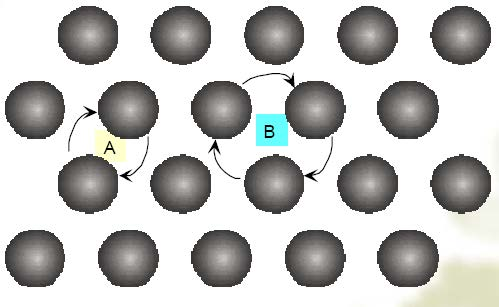
\includegraphics[width=0.5\textwidth]{fig/ring_diffusion.jpg}
                \caption{环行扩散的两种机制,其中A为直接交换,B为循环交换。}
                \label{环行扩散的两种机制}
            \end{figure}
        \subsection{空位扩散}
            \textbf{空位扩散}\index{空位扩散},对于晶体中存在的空位,空位周围的原子都是向空位进行扩散,
            扩散后形成新的空位。
        \subsection{挤列扩散}
            \textbf{挤列扩散}\index{挤列扩散}是在$n$个原子位置上挤进去一个原子,容纳了$n+1$个原子位置上挤进去一个原子,容纳了并作为
            一个整体沿挤列方向扩散。由于碱金属原子的压缩性较大,有可能形成这种组态。
    \section{Fick定律及其应用}
        \subsection{Fick第一定律}
            Fick 认为原子的扩散有具体的方向,应当从高浓度向低浓度扩散,以此得到了稳态下的Fick第一定律
            \begin{equation}
                J=-D\left( \frac{\partial c}{\partial x} \right)\label{Fick第一定律},
            \end{equation}
            上式称为\textbf{Fick第一定律}\index{Fick第一定律} ,其中 $J$为\textbf{扩散通量}\index{Fick第一定律!扩散通量},
            是某一时刻通过垂直于$x$轴的单位平面原子的通量;\textbf{扩散系数}\index{Fick第一定律!扩散系数},
            表示单位浓度梯度下的通量,上式表明,扩散方向与梯度方向相反。
            习惯上,\autoref{Fick第一定律}中各个量的单位为
            \begin{table}[ht]
                \centering
                \caption{Fick第一定律中各个物理量单位。}
                \label{Fick第一定律中各个物理量单位}
                \begin{tabular}{cc}
                    \toprule
                    物理量&单位\\
                    \midrule
                    $J$&\si{\g\per(\s\cdot\cm^2)}\\
                    $D$&\si{\cm^2\per\s}\\
                    $c$&\si{\g\per\cm^3}\\
                    $x$&\si{\cm}\\
                    \bottomrule
                \end{tabular}
            \end{table}
            
            对于三维空间,第一定律可以写作
            \begin{equation}
                J=-D\nabla c.
            \end{equation}
        \subsection{Fick第二定律}
            但是实际上,扩散通量$J$一般是不稳定的,伴随$x$变化,因此不同位置的浓度也会不同,
            对于$x_1$位置的$\dif x$厚度的体积元,单位时间的净通量为$J(x_1)-J(x_1+\dif x)$,
            其浓度改变速率为$\partial c/\partial t$,则有如下关系
            \begin{equation}
                \left( \frac{\partial c}{\partial t} \right)_{x_1}\dif x=J(x_1)-J(x_1+\dif x),
            \end{equation}
            当$\dif x\to0$时,有
            \begin{equation}
                J\left(x_{1}+\dif x\right)=J\left(x_{1}\right)+\left(\frac{\partial J}{\partial x}\right)_{x 1} \dif x
            \end{equation}
            所以有
            \begin{equation}
                \frac{\partial c}{\partial t}=-\frac{\partial J}{\partial x}=\frac{\partial}{\partial x}\left(D \frac{\partial c}{\partial x}\right),
            \end{equation}
            上式就是\textbf{Fick第二定律}\index{Fick第二定律}。
        
            一维情况下对于扩散系数$D$为常数的情况,Fick第二定律可以写作
            \begin{equation}
                D\left(\frac{\partial^{2} c}{\partial x^{2}}\right)=\frac{\partial c}{\partial t},
            \end{equation}
            对于扩散系数为变量的情况,Fick第二定律写作
            \begin{equation}
                \frac{\partial}{\partial x}\left[D\left(\frac{\partial c}{\partial x}\right)\right]=\frac{\partial c}{\partial t}.
            \end{equation}
            
            对于三维空间,在笛卡尔坐标系下,使用拉普拉斯算子,Fick第二定律可以写作
            \begin{equation}
                D\left(\frac{\partial^{2} c}{\partial x^{2}}+\frac{\partial^{2} c}{\partial y^{2}}+\frac{\partial^{2} c}{\partial z^{2}}\right)=\frac{\partial c}{\partial t}.
            \end{equation}

        \subsection{扩散方程的解}
            对于不同的类型,可以分为稳态扩散和非稳态扩散,其中\textbf{稳态扩散}\index{稳态扩散}
            是指空间各点的浓度不随时间发生变化,这种状态称为稳态扩散;\textbf{非稳态扩散}\index{非稳态扩散}是指
            空间中各点浓度随时间发生变化。
            \subsection{第一类稳态扩散}
                首先来看稳态扩散,假设扩散系数为常数,浓度不随时间发生变化。
                容器中间有金属薄板,薄板的一面保持高而恒定的浓度,另一面保
                持低而恒定的浓度,因此在金属板中存在浓度梯度。假设器壁不可渗透,
                经过一段时间,薄板中任一体积元,流入的和流出的通量相等,扩散达
                到稳定状态。
                
                此时的边界条件为$x=0$,$c=c_1$,$x=\Delta x$时,$c=c_0$,金属薄板的面积为$A$,
                总扩散通量为
                \begin{equation}
                    J_{\text{total}}=-AD\frac{\partial c}{\partial x},
                \end{equation}
                由于问题属于一维问题,可以将偏微分改为全微分
                \begin{equation}
                    J_{\text{total}}=-AD\frac{\dif c}{\dif x},
                \end{equation}
                两边同时乘以$\dif x$并在$0\to\dif x$范围内积分,有
                \begin{equation}
                    \int_{0}^{\Delta x}J_{\text{total}}\dif x=-\int_{c_{1}}^{c_{0}} A D \dif c
                \end{equation}
                得到
                \begin{equation}
                    J_{\text{total}}=\frac{AD(c_1-c_0)}{\Delta x}.
                \end{equation}

                这一类模型可以模拟钢铁真空脱气,假设金属表面溶解度与相接触的气体压力有关,对于
                双原子气体有
                \begin{equation}
                    c=S\sqrt{p},
                \end{equation}
                单位面积的扩散通量就可以写作
                \begin{equation}
                    J=\frac{D S\left(\sqrt{p_{1}}-\sqrt{p_{0}}\right)}{\Delta x}.
                \end{equation}
            \subsubsection{第二类稳态扩散}
                这类问题扩散是指空间各点的浓度不随时间发生变化,但是扩散系数$D$不是常数。
                有人利用这一特点模拟了碳在$\gamma$铁中的扩散过程并测量了扩散系数。

                将长度为$l$、半径为$r$的薄壁铁管在\SI{1000}{\celsius}下退火,管内
                是渗碳气氛,关外是脱碳气氛,当时间最够长时,壁管内各点的碳浓度不再随时间而变,
                也就是
                \begin{equation}
                    \frac{\partial c}{\partial t}=0.
                \end{equation}
                达到稳定状态后,设$t$时间内通过管壁的碳量为$q$,则单位时间通过
                的碳量$q/t$为常量。因而,单位时间流入或流出单位面积的通量为
                \begin{equation}
                    J=\frac{q}{2\pi lt},
                \end{equation}
                根据\autoref{Fick第一定律}可得
                \begin{equation}
                    \frac{q}{2\pi lt}=-D\frac{\dif c}{\dif r},
                \end{equation}
                解得
                \begin{equation}
                    q=-D\left( 2\pi lt \right)\frac{\dif c}{\dif \ln r},
                \end{equation}
                式中,$q$,$l$,$t$以及碳沿管壁的径向分布都可以测量,扩散系数$D$
                可以由$c$对$\ln r$的斜率确定。

            \subsubsection{第一类非稳态扩散}
                这种情况是空间各点的浓度随时间发生变化,但是$D$为常数的情况,
                此时的Fick第二定律可以写作
                \begin{equation}
                    \frac{\partial c}{\partial t}=D \frac{\partial^{2} c}{\partial x^{2}}.
                \end{equation}
                这一公式可以解决两种模型,分别为\textbf{瞬时平面源}\index{瞬时平面源}和
                \textbf{一维半无限模型}\index{一维半无限模型}(也称为叠加法)。

                对于瞬时平面源模型,假设两块足够长的相同纯金属,其中
                一块端面上涂上同位素(作为扩散面源),对接起来组成扩散偶,假设扩散系数为常数
                Fick第二定律的解的形式为
                \begin{equation}
                    c=\frac{A}{\sqrt{t}} \exp \left(-\frac{x^{2}}{4 D t}\right),
                \end{equation}
                式中$A$为待定系数。由于扩散总量一定,为$M$,也就是
                \begin{equation}
                    \int_{-\infty}^{\infty} c(x, t) \mathrm{d} x=M,
                \end{equation}
                可以解得
                \begin{equation}
                    c(x, t)=\frac{M}{2 \sqrt{\pi D t}} e^{-\frac{x^{2}}{4 D t}}
                \end{equation}

                对于另一种模型,则是假设一块无限长的金属,$x<0$为扩散源,$x>0$为被扩散物质。
                首先求解单位体积元扩散对$x>0$的某一点的影响,该点的总浓度就是所有体积元作用的总和。
                求解过程相对复杂,这里直接给出结果
                \begin{equation}
                    c(x, t)=\frac{c_{0}}{2}\left[1-\operatorname{erf}\left(\frac{x}{2 \sqrt{D t}}\right)\right]
                \end{equation}
                其中$\operatorname{erf}$为误差函数,其有数值表可以查阅。
                假设初始浓度为$c=c_0$,扩散时,表面浓度恒定为$c=c_s$,则上式可以写作
                \begin{equation}
                    c(x,t)=c_0+(c_s-c_0)\left[ 1-\operatorname{erf}\left( \frac{x}{2\sqrt{Dt}} \right) \right],
                \end{equation}
                这一公式适用于工业上工件的渗碳过程。

                这里还有一个概念性的常用关系式,当某一处的浓度满足
                \begin{equation}
                    \frac{c-c_{0}}{c_{s}-c_{0}}=\frac{1}{2},
                \end{equation}
                该处对应的位置为
                \begin{equation}
                    x_{\frac{1}{2}}=\sqrt{Dt},
                \end{equation}
                这一位置的$x$称为\textbf{半浓度深度}\index{Fick第二定律!半浓度深度},记作$x_{1/2}$,
                对与任意时间都成立。

                对于温度改变的系统,测量此时的\textbf{扩散系数}\index{Fick第二定律!扩散系数} ,可以发现其与温度有明显的关系,一般可以写作
                \begin{equation}
                    D=D_0\exp\left( -\frac{Q}{RT} \right),
                \end{equation}
                上式称为\textbf{Arrhenius关系}\index{Fick第二定律!扩散系数!Arrhenius关系},其中$Q$为
                扩散激活能,式中$Q$、$D_0$与温度无关,与成分、结构有关。
            \subsubsection{第二类非稳态扩散}